The main idea of logistic regression is to predict from a set of discrete binary values (ex: have cancer or not [0, 1]). In order to acomplish that, we use a linear function (Decision boundary, can be non-linear) to map all predictions greater than 0.5 as 1 and all less than 0.5 as a 0. This \textbf{prediction} is done by a \textbf{sigmoid} ($g(x)$) function that normalizes the output of the \textbf{Decision boundary} ($\theta^Tx$) to just 1 or 0.

So in conclusion, there is a \textbf{hypotheses} ($h_{\theta}(x)$) function that is the sigmoid ($g(x)$) function applied to the Decision boundary; and the \textbf{goal} is to find the most accurate parameters for the Decision boundary ($\theta^Tx$).

\subsection{Concepts}
\subsubsection{Sigmoid function}
Also called \textit{Logistic function}, maps any real number to the (0, 1) interval, making it useful for transforming an arbitrary-valued function into a function better suited for classification. The function has this form:

\begin{align}
	g(z) & = \frac{1}{1 + e^{-z}}
\end{align}

And looks like:
\begin{figure}[h]
    \centering
    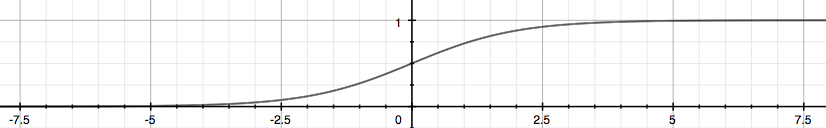
\includegraphics[width=1\textwidth]{sigmoid-function}
    \caption{Sigmoid function}
    \label{fig:sigmoid}
\end{figure}

\subsubsection{Hypotheses function}
This hypotheses function will predict, using some input data ($x_i$) and a set of precomputed coefficients ($\theta$), a number between 0 and 1.

$$0 \le h_{\theta}(x) \le 1$$

In order to achieve this, we use the sigmoid function to map our output to 0 - 1 interval on the decision boundary. The function has this form:

\begin{align}
	h_{\theta}(x) & = g(\theta^Tx) = g(X\theta)
\end{align}

$$h_{\theta}(x) = \frac{1}{1 + e^{-\theta^Tx}}$$

The result of this function can be interpreted as \textit{the probability that the output is 1}. For example, $h_{\theta}(x)=0.7$ gives us a probability of 70\% that our output is 1. Our probability that our prediction is 0 is just the complement of our probability that it is 1 (e.g. if probability that it is 1 is 70\%, then the probability that it is 0 is 30\%).


\subsubsection{Decision boundary}
This function describes the line (can be polynomial) that determines the limit of the features in order to predict wether 0 or 1. The representation for the decision boundary is:

$$\theta^Tx$$


In order to visualize it, we need to separate the ones that are $y = 0$ and the ones that are $y = 1$, then plot all features. But all axis must be the features ($x^{(j)}$) displayed separately the \textit{0's} from the \textit{1's}


And it can have many forms, also polynomial.


\begin{figure}[h]
	\begin{multicols}{2}
	\centering
	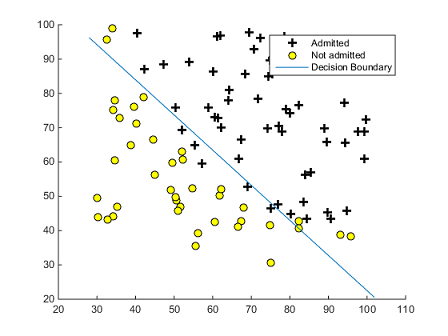
\includegraphics[width=0.4\textwidth]{decision-boundary}
	\caption{Linear Decision boundary}
	\label{fig:decision-boundary}

	\centering
	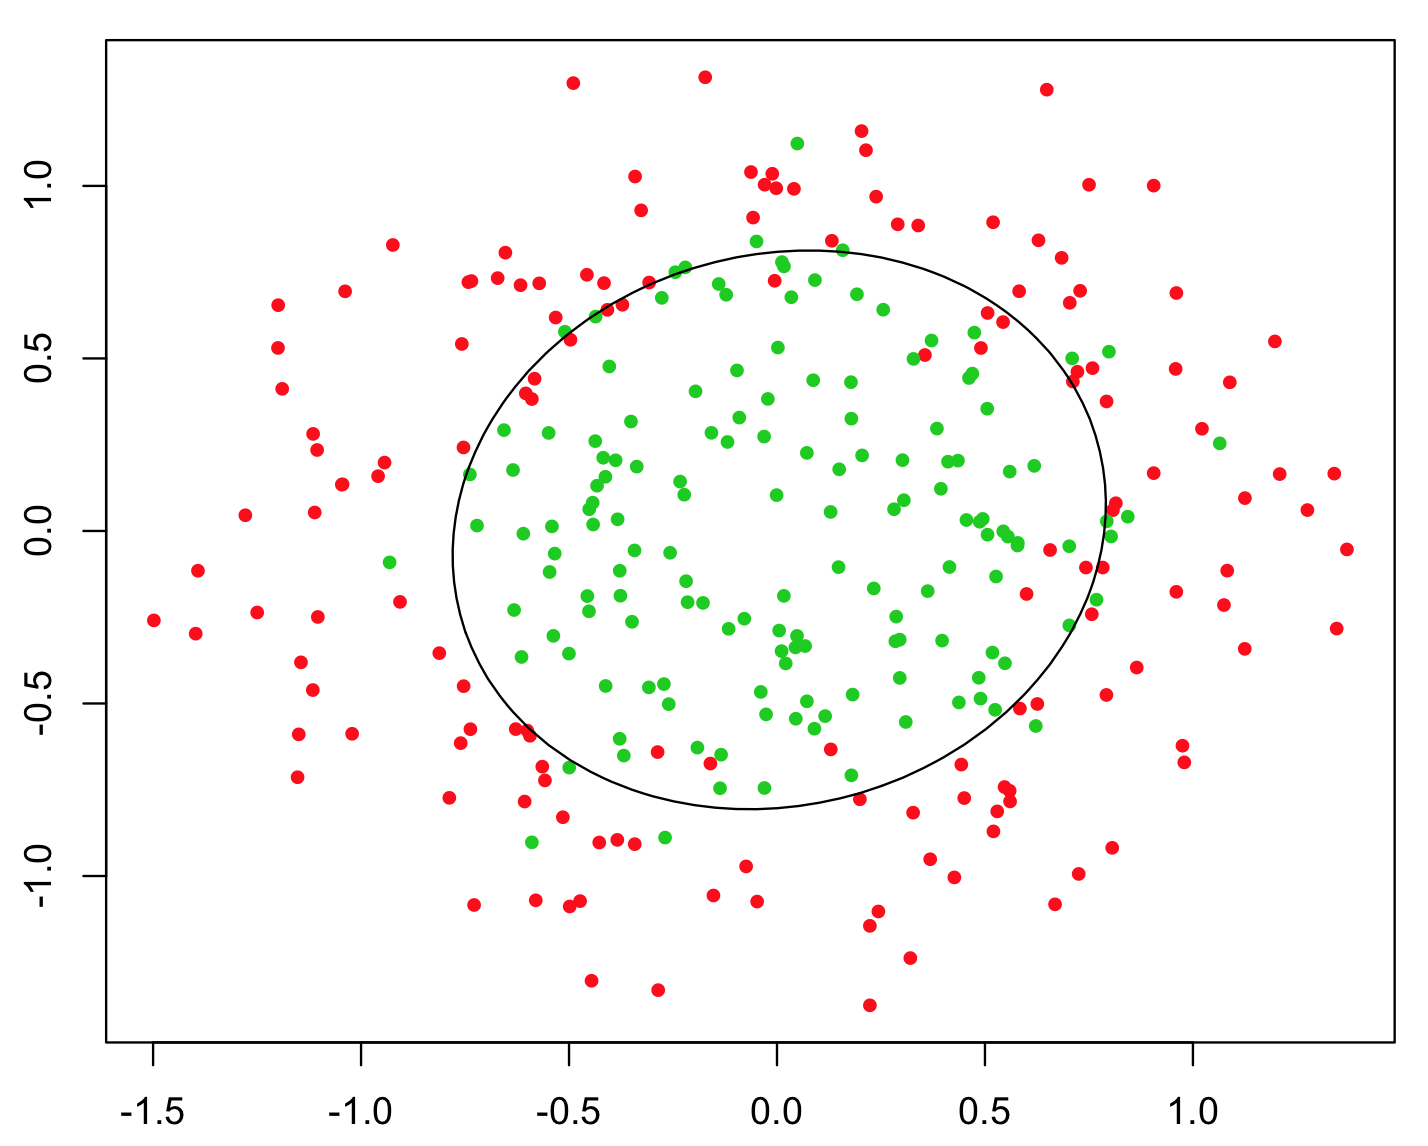
\includegraphics[width=0.4\textwidth]{decision-boundary-2}
	\caption{Cuadratic Decision boundary}
	\label{fig:decision-boundary-2}
	\end{multicols}
\end{figure}



We can interpret the output of the hypotheses function as:

\begin{align*}
	h_{\theta}(x) \ge 0.5 \to  y = 1 \\
	h_{\theta}(x) < 0.5 \to  y = 0
\end{align*}

If we observe Figure \ref{fig:sigmoid} we can observe that in order to get $g(z) \ge 0.5$ we need $z$ to be greater than $0$, in other words:

\begin{align*}
	& h_{\theta}(x) = g(\theta^Tx) \ge 0.5 \to  y = 1 \\
	& \text{when } z = \theta^Tx \ge 0
\end{align*}

Remember:

\begin{align*}
	& z = 0, e^0 = 1 \Rightarrow g(z) = 1/2 \\
	& z \to \infty, e^{\infty} \to 0 \Rightarrow g(z) = 1 \\
	& z \to -\infty, e^{-\infty} \to 0 \Rightarrow g(z) = 0 \\
\end{align*}

\subsection{Cost Function}
We cannot use the same cost function that we use for linear regression because the Logistic Function will cause the output to be wavy, causing many local optima. In other words, it will not be a convex function.

\begin{align*}
	& J(\theta) = \frac{1}{m} \sum_{i=1}^{m}Cost(h_{\theta}(x^{(i)}), y^{(i)}) \\
	& Cost(h_{\theta}(x), y) = -log(h_{\theta}(x)) \qquad\qquad\qquad \text{if } y = 1 \\
	& Cost(h_{\theta}(x), y) = -log(1 - h_{\theta}(x)) \qquad\qquad \text{if } y = 0 \\
\end{align*}

The interpretation for this
\begin{figure}[h]
	\begin{multicols}{2}
	\centering
	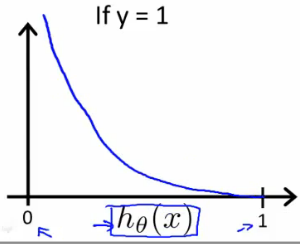
\includegraphics[width=0.4\textwidth]{logistic-regression-cost}
	\caption{$-log(h_{\theta}(x))$}
	\label{fig:logistic-regression-cost}

	\centering
	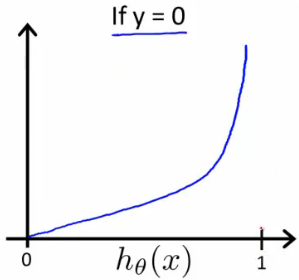
\includegraphics[width=0.4\textwidth]{logistic-regression-cost-2}
	\caption{$-log(1 - h_{\theta}(x))$}
	\label{fig:logistic-regression-cost-2}
	\end{multicols}
\end{figure}

But there is a much simpler and compat way to represent that conditional:

\begin{align}
	J(\theta) = \frac{1}{m} \sum_{i=1}^{m} -y^{(i)}log(h_{\theta}(x^{(i)})) - (1-y^{(i)})log(1 - h_{\theta}(x^{(i)}))
\end{align}

